 % !TEX program = lualatex
\documentclass[xcolor={x11names, table}, compress]{beamer}

\usepackage{xcolor}
\usepackage{fontspec}
\usepackage{pgfplots}
\usepackage{tikz}
\usepackage{amsmath, amssymb, amsfonts}
\usepackage{bm}
\usepackage{eso-pic}
\usepackage{graphicx}
\usepackage{verbatim}

\pgfplotsset{compat=1.15}
\usetikzlibrary{positioning, shapes, calc, arrows}
\hypersetup{pdfstartview={Fit}}

%% Beamer Layout %%%%%%%%%%%%%%%%%%%%%%%%%%%%%%%%%%
\useinnertheme{default}
\usepackage[T1]{fontenc}
\usefonttheme{professionalfonts}  % Font for math

\setbeamerfont{frametitle}{}

\definecolor{BHKpresentationDark}{RGB}{114,133,176}
\definecolor{BHKpresentationDarkGrey}{RGB}{103,116,128}
\definecolor{BHKblue}{RGB}{51,105,153}

\setbeamerfont{title like}{shape=\scshape}
\setbeamercolor*{frametitle}{fg=BHKpresentationDark} 
\setbeamercolor*{lower separation line head}{bg=BHKblue} 
\setbeamercolor*{normal text}{fg=BHKpresentationDarkGrey,bg=white} 
\setbeamercolor*{alerted text}{fg=BHKblue} 
\setbeamercolor*{example text}{fg=black} 
\setbeamercolor*{item}{fg=BHKpresentationDark,bg=gray} 
\setbeamercolor{enumerate item}{fg=BHKpresentationDark}
\setbeamercolor*{structure}{fg=black} 
\setbeamercolor*{palette tertiary}{fg=black,bg=black!10} 
\setbeamercolor*{palette quaternary}{fg=black,bg=black!10} 
\setbeamercovered{transparent}

\setbeamertemplate{navigation symbols}{}
\setbeamertemplate{footline}{%
    \begin{beamercolorbox}[wd=\paperwidth]{footlinecolor}
        
\includegraphics[width=\textwidth]{bar_footline.pdf}
    \end{beamercolorbox}%
}

\setbeamertemplate{frametitle}[default][center]
\setbeamertemplate{caption}[numbered]
\setbeamertemplate{section in toc}[sections numbered]
\setbeamertemplate{subsection in toc}[subsections numbered]


\newcommand{\insertsec}{\thesection.~\insertsection}
\newcommand{\insertsubsec}{\thesection.\thesubsection~\insertsubsection}

%%%%%%%%%%%%%%%%%%%%%%%%%%%%%%%%%%%
%% Start of document %%%%%%%%%%%%%%
%%%%%%%%%%%%%%%%%%%%%%%%%%%%%%%%%%%

\begin{document}
%%%% title slide %%%%%
{\setbeamertemplate{footline}{} 
    \begin{frame}
        \vspace{-1.5cm}
        \hfill\makebox[0.2\paperwidth]{
\includegraphics[width=0.4\textwidth]{logo_wtext}}
        \begin{flushleft}
            \hspace{-1cm}
\includegraphics[width=0.8\textwidth, height=0.4em]{title_line.pdf}\hfill
            
            \title{
                \begin{flushleft}{
                    \huge \color{BHKpresentationDark} 
                    Lab Meeting
                } 
                \end{flushleft}
            }
            
            \vspace{-.5cm}
            \date{Monday 19th of March, 2018}
            \author[Joan]{\begin{flushleft}\vspace{-1cm} Joan Marcè i Igual\end{flushleft}}
            \titlepage{}
        \end{flushleft}
    \end{frame}
}

\begin{frame}{Table of Contents}
	\tableofcontents
\end{frame}


\section{What have I done?}

\begin{frame}{\insertsec}
    
    I've been doing Neural Networks related courses at Coursera

    \begin{center}
        
\includegraphics[width=.5\textwidth]{images/coursera_logo}
    \end{center}

    \begin{itemize}
        \item Neural Networks and Deep Learning (\emph{94.3\%})
        \item Improving Deep Neural Networks: Hyperparameter tuning, Regularization and 
        Optimization (\emph{97.8\%})
        \item Convolutional Neural Networks (\emph{94.4\%})
    \end{itemize}
\end{frame}



\section{DeepSurv}

\begin{frame}{\insertsec}
    Paper published by Jared L.Katzman \emph{et al.} (2017) using a deep learning approach for
    the Survival Prediction problem.
    
    \begin{itemize}
        \item Shows an application of deep learning to survival analysis
        \item It uses this deep learning model to create a personalized treatment 
        recommender system
        \item Uses the Cox Proportional Hazards Model
    \end{itemize}
    
\end{frame}

\begin{frame}{The Survival Prediction Problem}
    Survival data has three elements: patient's baseline data \( x \), a failure event 
    time \( T \) and an event indicator \( E \).
    
    There's the survival function (\( S(t) = \Pr(T > t) \)) and the hazard function
    \( \lambda(t) \):
    \[
        \lambda(t) = \lim_{\delta \rightarrow 0} 
        \frac{\Pr(t \le T < t + \delta | T \ge t)}{\delta} 
    \]

    Given baseline data \( x \) the hazard function is assumed to have the form:
    \[
        \lambda(t | x) = \lambda_0 (t) \cdot e^{\bm{h(x)}}
    \]
\end{frame}

\begin{frame}{Linear Survival Models}
Cox Proportional Hazards model estimates that the risk function \( h(x) \) is linear 
\( \hat{h}_{\beta}(x) = \beta^T x \). The partial likelihood, parameterized by \( \beta \) is 
defined:

\[
    L_c (\beta) = \prod_{i:E_i = 1} \frac{\exp(\hat{h}_{\beta}(x_i))}
    {\sum_{j \in \mathfrak{R}(T_i)} \exp(\hat{h}_{\beta}(x_j))}
\]
\[
    \mathfrak{R}(t) = \{i: T_i \ge t\}
\]
    
\end{frame}

\begin{frame}{Nonlinear survival models}
The used loss function is the following one
    
\[
    l(\theta) := -\sum_{i:E_i = 1} \left(
    \hat{h}_{\theta}(x_i) - \log \sum_{j \in \mathfrak{R}(T_i)} e^{\hat{h}_{\theta} (x_j)}
    \right)
\]
\end{frame}

\section{Google: Learning Hand-Eye Coordination for Robotic Grasping}

\begin{frame}{\insertsec}
Paper published by Sergey Levine \emph{et al.} (2016).
Its objective is for a robot to learn how to grab pieces by using only image data and a movement
and rotation vector.

\begin{center}
    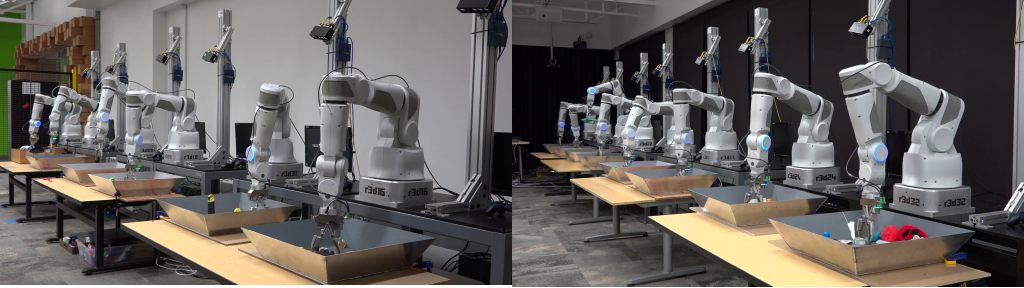
\includegraphics[width=.9\textwidth]{images/google_robot}
\end{center}
\end{frame}


\begin{frame}
Network with both image input and scalar input, each value is repeated 
\(img.width \times img.height\) times to match the CNN size.
\begin{center}
    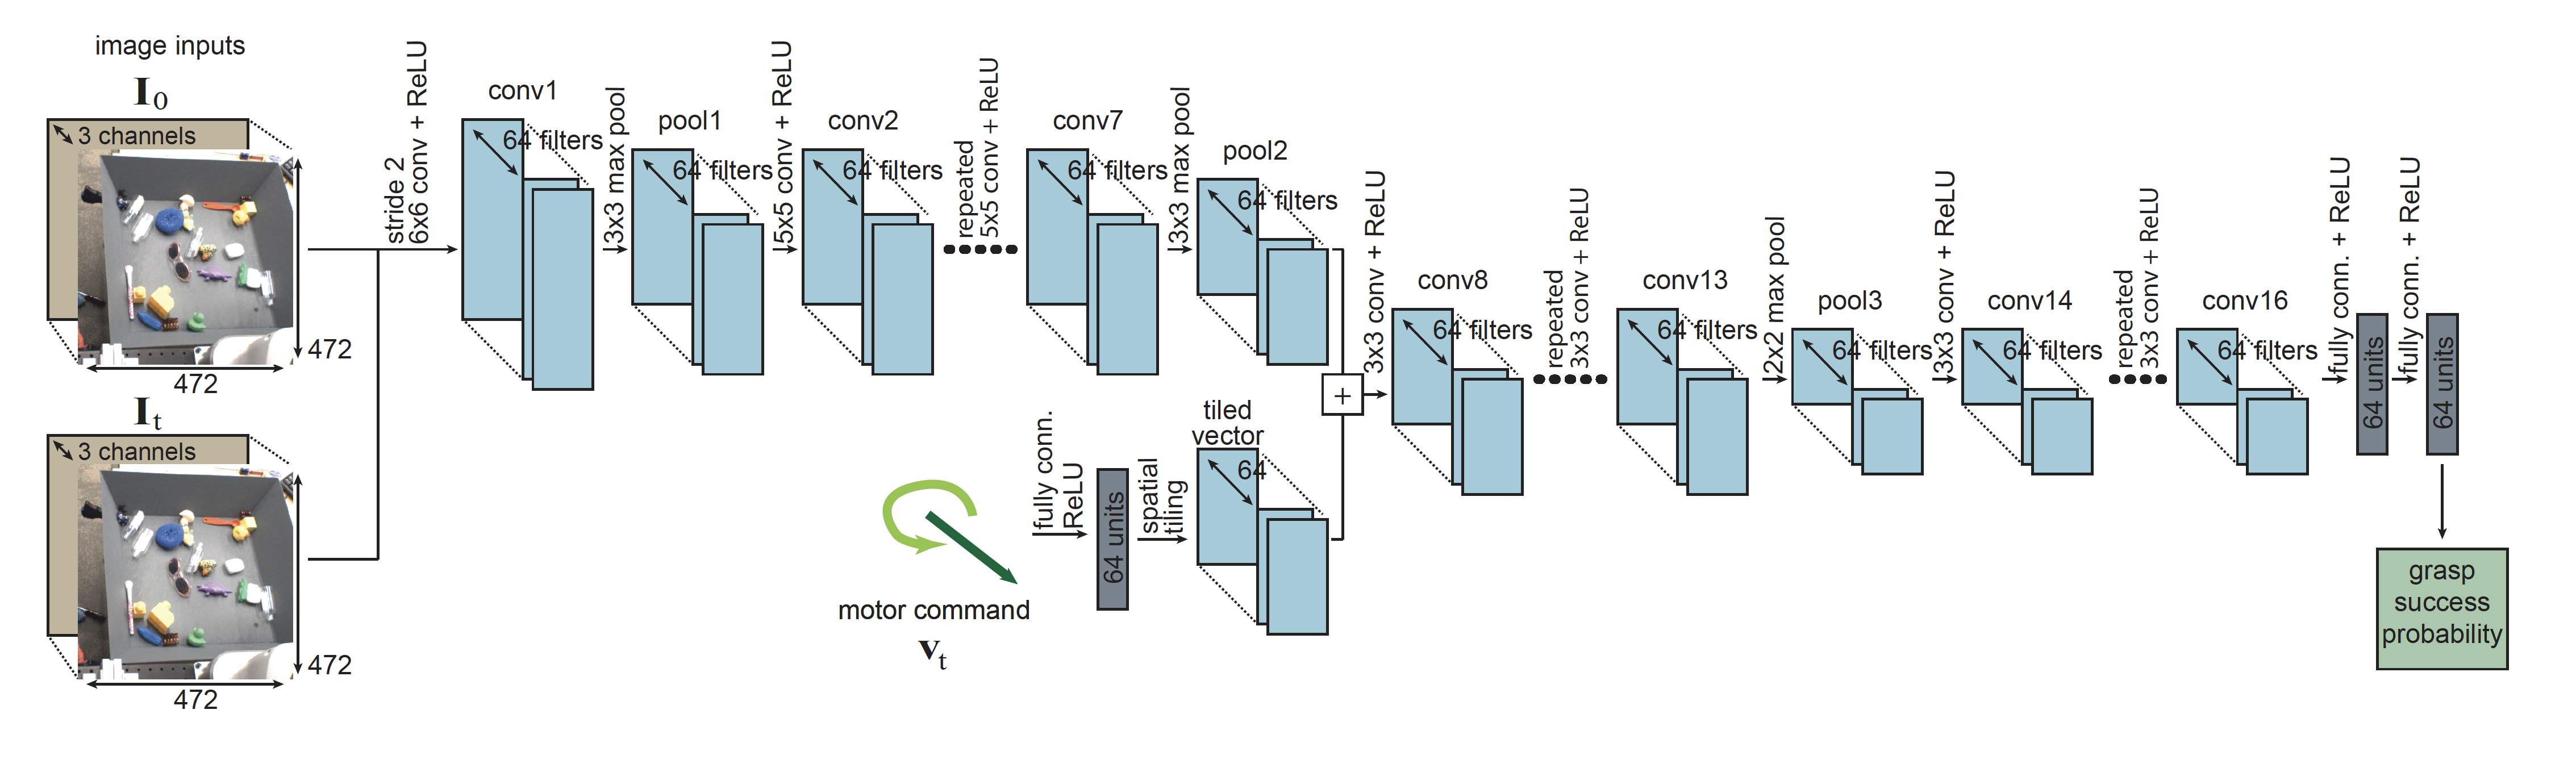
\includegraphics[width=\textwidth]{images/google_robot_network}
\end{center}
\end{frame}
\section{Proposal}

\begin{frame}{\insertsec}
\begin{itemize}
  \item Use Cox Proportional Hazards model like DeepSurv
  \item Use a Convolutional Neural Network 3D. If it does not work well then:
  \begin{itemize}
    \item Select best slice
    \item Use a Convolutional Neural Network 2D
  \end{itemize}
  \item Use radiomics features
  \item Combine both radiomics features (scalar values) and images using a similar model 
  like the Hand-Eye Coordination paper
\end{itemize}
\end{frame}

\begin{frame}{\insertsec}
  \begin{columns}
    \begin{column}{.5\textwidth}
      \begin{itemize}
        \item Start with a simple example:
        \begin{itemize}
          \item 1 CNN layer
          \item 1 FN layer
          \item Spatial Filling
          \item Combine layers
          \item 1 CNN layer
          \item 1 FC layer
        \end{itemize}
    \end{itemize}
  \end{column}
  \begin{column}{.5\textwidth}
    
    \begin{center}
        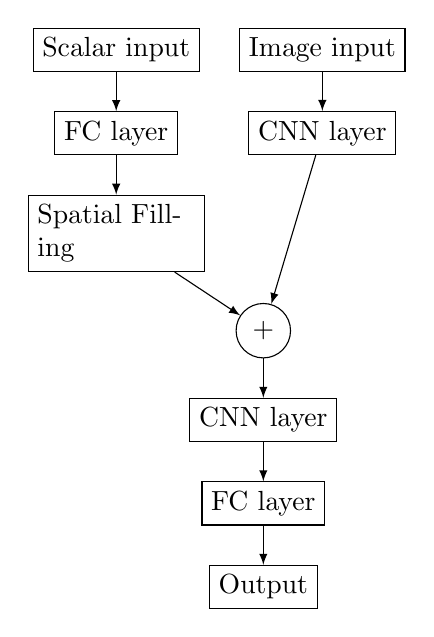
\begin{tikzpicture}[node distance = .5cm]
            \tikzstyle{neuron}=[rectangle, draw=black]
            \node [neuron] (I-Image) at (0, 0) {Image input};
            \node [neuron, left = of I-Image] (I-Scalar) {Scalar input};

            \node [neuron, below = of I-Image] (CNN-01) {CNN layer};
            \node [neuron, below = of I-Scalar] (FC-01) {FC layer};
            \node [neuron, below = of FC-01, text width = 2cm] (aug) {Spatial Filling}; 

            \node [circle, draw = black, below right = .7 of aug] (join) {\(+\)};

            \node [neuron, below = of join] (CNN-02) {CNN layer};
            \node [neuron, below = of CNN-02] (FC-02) {FC layer};

            \node [neuron, below = of FC-02] (output) {Output};

            \draw [-latex] (I-Image) -- (CNN-01);
            \draw [-latex] (I-Scalar) -- (FC-01);
            \draw [-latex] (FC-01) -- (aug);
            \draw [-latex] (aug) -- (join);
            \draw [-latex] (CNN-01) -- (join);
            \draw [-latex] (join) -- (CNN-02);
            \draw [-latex] (CNN-02) -- (FC-02);
            \draw [-latex] (FC-02) -- (output);

        \end{tikzpicture}

    \end{center}
  \end{column}
\end{columns}
\end{frame}

\end{document}